\section{Ziel}
\label{sec:Ziel}
Trifft ein nach der geometrischen Optik definierter Lichtstrahl auf einen Spalt oder ein Hindernis, weicht er von seinem ursprünglichem Weg ab und wird gebeugt.
Versuchsziel ist es, die Spaltbreiten verschiedener Blenden sowohl über die Intensität einer Beugungsfigur, als auch per Mikroskop zu bestimmen um anschließend die unterschiedlichen Methoden miteinander vergleichen zu können.


\section{Theorie}
\label{sec:Theorie}
Wird Licht an einem Spalt gebeugt, entsteht ein Beugungsbild. Dieses charakteristische Muster kann mit dem Prinzip von \textsc{Huygens} erklärt werden. 
Es besagt, dass von jedem Punkt einer Welle kugelförmige Elementarwellen ausgehen. 
Diese treten auch am Spalt auf und interferieren miteinander.
Dabei  erzeugen sie durch konstruktive und destruktive Interferenz die auftretenden Intensitätsmaxima und -minima des Beugungsbildes.
Die Intensität $I$ hängt stark vom Beugungswinkel $\varphi$, d.h. der Richtung, in die die Strahlen gebeugt werden, ab.
Mathematisch kann die Beugung durch zwei Näherungen \\ -- \textsc{Fresnel}- und \textsc{Fraunhofer}-Beugung -- beschrieben werden, die in Abbildung \ref{fig:naeherung} dargestellt sind.

\begin{figure}
	\centering
	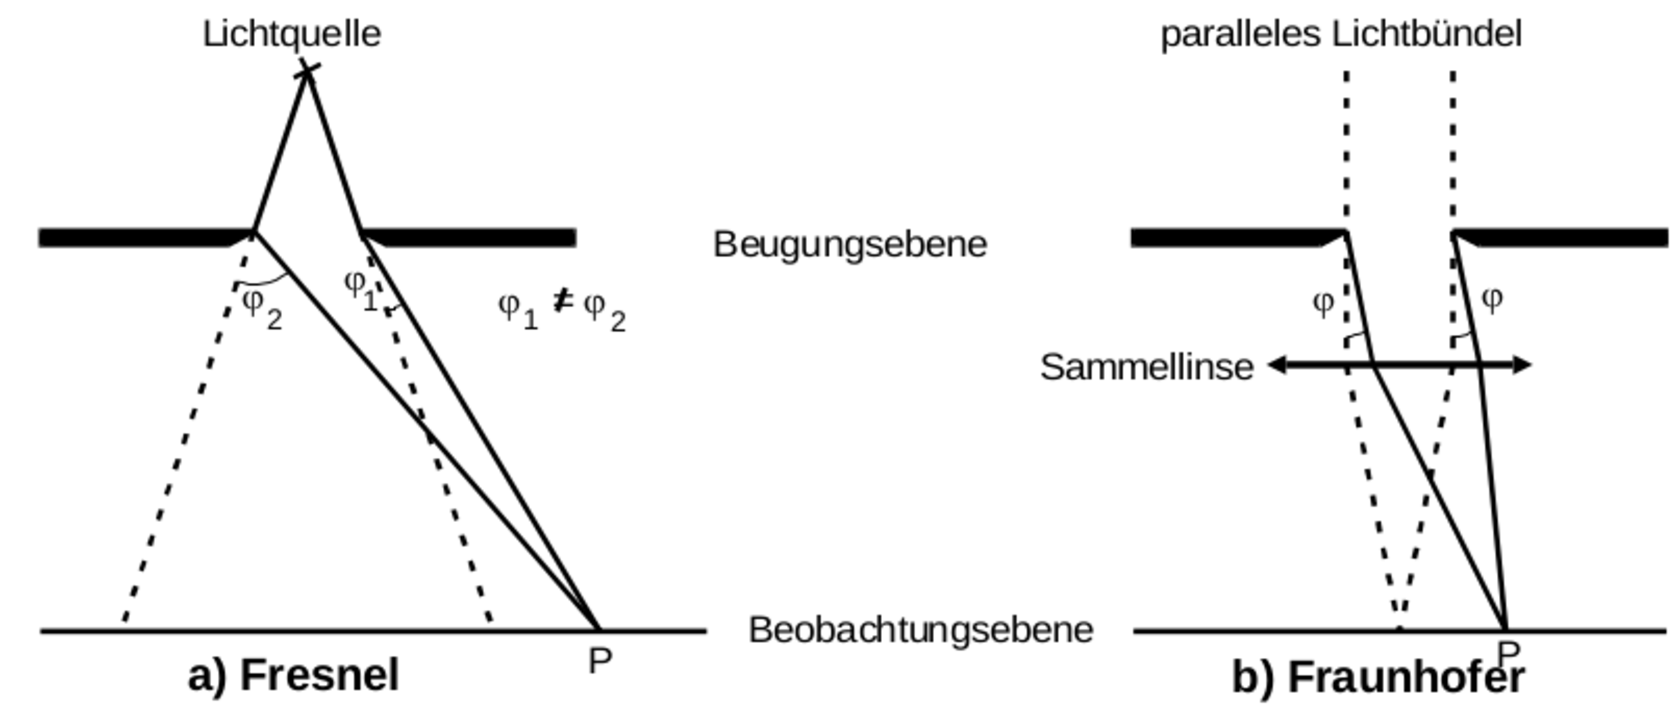
\includegraphics[width=0.7\textwidth]{Bilder/Naeherungen.pdf}
	\caption{Skizze beider Näherungen.\cite{V406}}
	\label{fig:naeherung}
\end{figure}

Befinden sich Lichtquelle und Beobachtungspunkt in endlicher Entfernung zueinander, werden divergente Strahlenbündel am Spalt unter verschiedenen Winkeln $\varphi_1$ und $\varphi_2$ gebeugt und interferieren in einem Punkt $P$, dies ist die \textsc{Fresnel}-Beugung.
Den Gegensatz dazu bildet die \textsc{Fraunhofer}-Beugung. Hier befinden sich Lichtquelle und Beobachtungspunkt unendlich weit voneinander entfernt. 
Dies hat zur Folge, dass die am Spalt ankommenden Lichtstrahlen parallel verlaufen. 
Im Beobachtungspunkt interferieren deshalb nur die Strahlen, die unter dem selben Winkel $\varphi$ gebeugt wurden. 
Im weiteren Verlauf soll die \textsc{Fraunhofer}-Näherung genutzt werden.



\subsection{Beugung am Parallelspalt}

\begin{equation}
	A(z,t)=A_0\exp{\left(i\left(\omega t -\frac{2\pi z}{\lambda}\right)\right)}
\end{equation}
des im Winkel $\varphi$ gebeugten Lichts, indem über die Spaltöffnung -- mathematisch als Aperturfunktion bezeichnet-- integriert wird. 

\begin{figure}
	\centering
	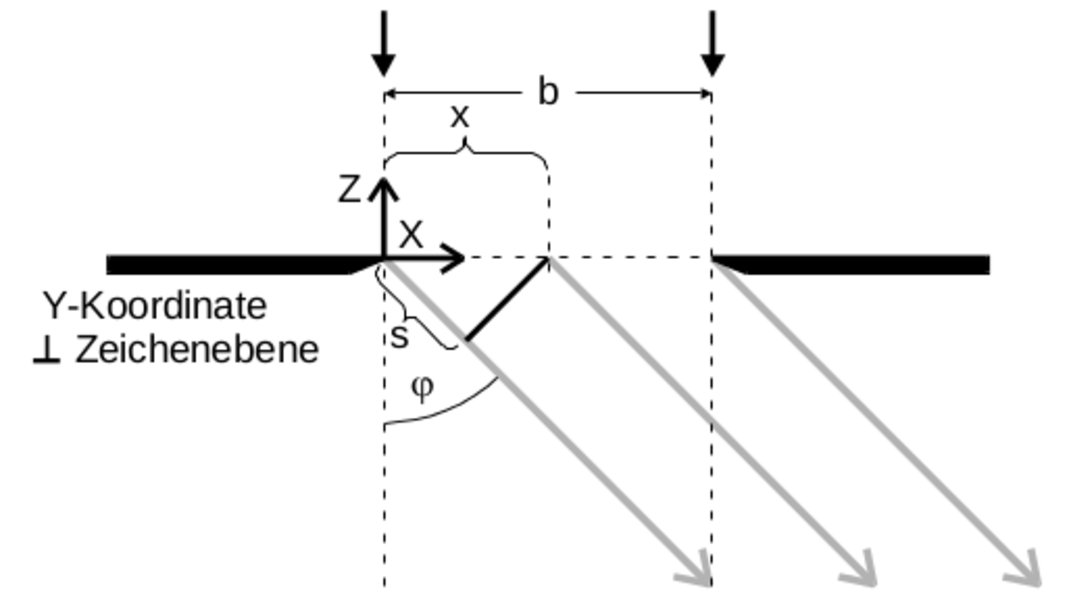
\includegraphics[width=0.6\textwidth]{Bilder/Einfachspalt.pdf}
	\caption{Beugung am Einzelspalt.\cite{V406}}
	\label{fig:einzelspalt}
\end{figure}

Weisen die Wellenfronten wie in Abbildung \ref{fig:einzelspalt} einen Wegunterschied $s$ auf, weil sie um den Abstand $x$ voneinander entfernt sind, ergibt sich zwischen ihnen eine Phasendifferenz von

\begin{equation}
	\sigma=\frac{2\pi s}{\lambda}=\frac{2\pi x \sin{\varphi}}{\lambda}.
\end{equation}

Damit resultiert die Amplitude

\begin{equation}
	B(z,t,\varphi)=A_0\exp{\left[i\left(\omega t -\frac{2\pi z}{\lambda}\right)\right]}\cdot \exp{\left(\frac{i b \pi \sin{\varphi}}{\lambda}\right)}\cdot\frac{\lambda}{\pi\sin\varphi}\sin{\left(\frac{\pi b \sin\varphi}{\lambda}\right)}.
	\label{eq:A}
\end{equation}
Bedeutsam für die Versuchsauswertung ist nur der letzte Faktor in Gleichung \eqref{eq:A}; die Exponentialfunktionen beschreiben Zeit- und Ortsabhängigkeit der Amplitude $B$ bzw. stellen einen Phasenfaktor dar, welcher die nachfolgend betrachtete zeitlich gemittelte Intensität

\begin{equation}
	I(\varphi)\propto B(\varphi)²={A_0}²b²\left(\frac{\lambda}{\pi b \sin{\varphi}}\right)²\cdot \sin²{\left(\frac{\pi b \sin\varphi}{\lambda}\right)}
	\label{eq:regress1}
\end{equation}

nicht beeinflusst.
Die Höhe der Intensitätsmaxima nimmt mit $\varphi²$ ab; Nullstellen -- also Intensitätsminima -- befinden sich an den Stellen

\begin{equation}
	\sin\varphi_n=\pm n\frac{\lambda}{b},\,n=1,2,.. .
\end{equation}

\begin{figure}
	\centering
	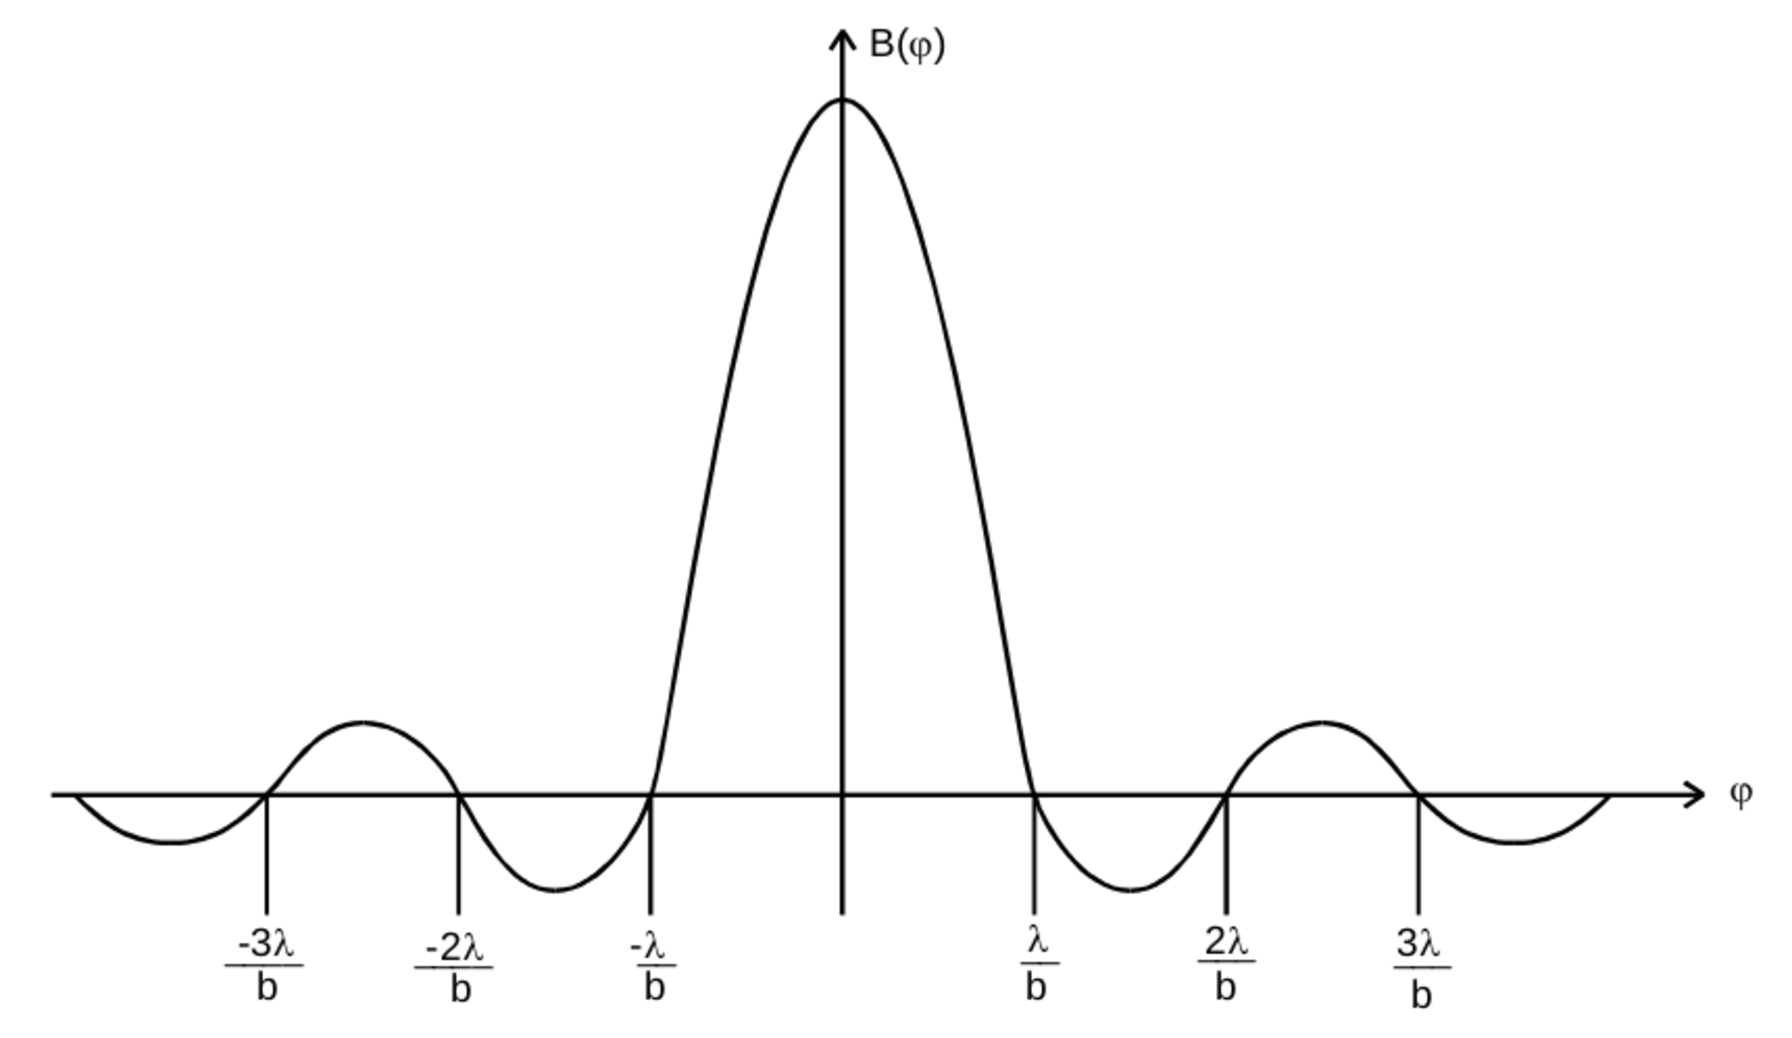
\includegraphics[width=0.7\textwidth]{Bilder/Beugungsbild.pdf}
	\caption{Beugungsbild des Einzelspaltes.\cite{V406}}
\end{figure}

\subsection{Beugung am Doppelspalt}
\begin{figure}
	\centering
	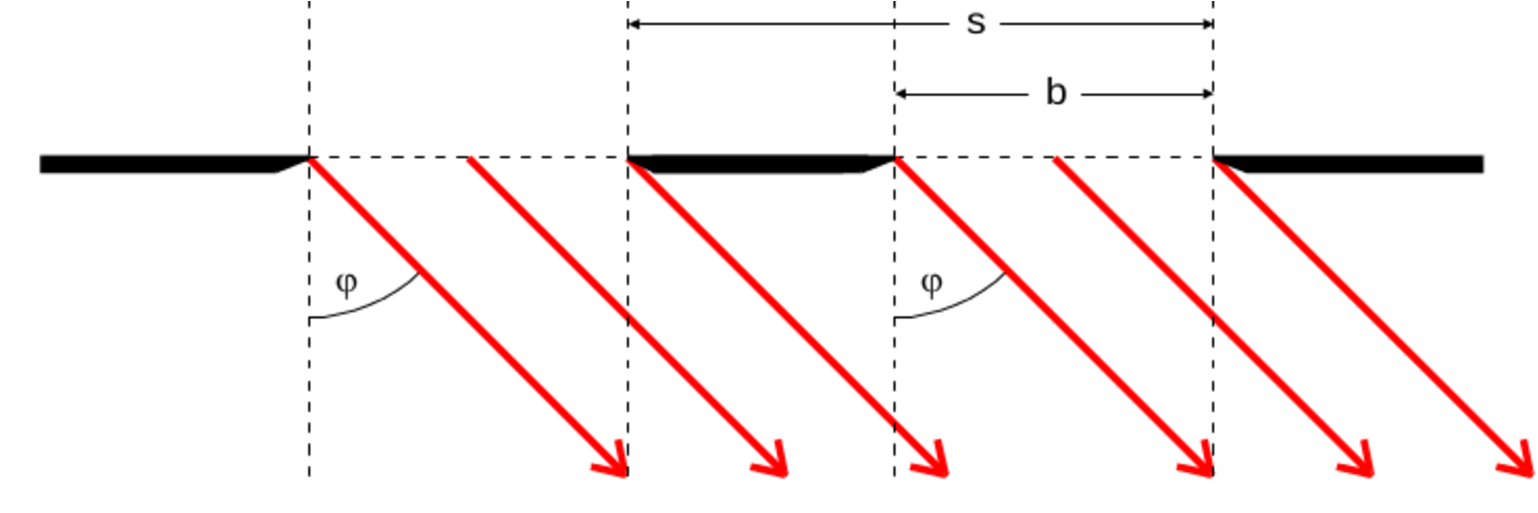
\includegraphics[width=0.6\textwidth]{Bilder/Doppelspalt.pdf}
	\caption{Beugung am Doppelspalt.\cite{V406}}
\end{figure}

Die Beugungsfigur ergibt sich durch die Überlagerung zweier Einzelspalte und einer Cosinus-Verteilung:

\begin{equation}
	I(\varphi)\propto B(\varphi)²=4\cos²{\left(\frac{\pi s \sin\varphi}{\lambda}\right)}\left(\frac{\lambda}{\pi b \sin\varphi}\right)²\sin²{\left(\frac{\pi b \sin\varphi}{\lambda}\right)}.
	\label{eq:regress2}
\end{equation}

Neben den Minima der Einzelspalte erscheinen zusätzlich Minima an 

\begin{equation}
	\varphi(k)=\arcsin²{\left(\frac{2k+1}{2s}\right)}\lambda,
\end{equation}

den Nullstellen der Cosinus-Funktion.
Allgemein wird die Funktion $B(\varphi)$ beschrieben als die \textsc{Fourier}-Transformierte

\begin{equation}
	g(\epsilon)=\int _{-\infty}^\infty { f(x)\exp{\left(ix\epsilon\right)} dx}
\end{equation}
der Amplitudenverteilung der Welle in der Beugungsebene.
Dabei werden alle am Spalt auftretenden Elementarwellen aufsummiert und mit einer Exponentialfunktion als Phasenfaktor versehen.
